\chapter{Continuous Random Variables}

\section{Probability Density Function}

Recall that a random variable is \bred{continuous} if it can take on values on an interval of real numbers. For example, 

\begin{itemize}
    \item The mass of a randomly selected salmon in kilograms 
    \item The horizontal distance a figure skater travels on a specific type of jump in metres 
    \item The random elapsed time between football plays in seconds
\end{itemize}

\begin{definition}[Probability Density Function]
    The \term{probability density function} (PDF) of a continuous random variable $X$ is a function $f(x)$ that has the following properties.

    \begin{enumerate}
        \item $f(x) \ge 0$ for all $x$ in the support of $X$
        \vspace{0.5em}
        \item $\int_{-\infty}^{\infty} f(x) \,dx = 1$
        \item $P(a \le X \le b) = \int_a^b f(x) \,dx$
    \end{enumerate}
\end{definition}

Note that unlike in the discrete case, the density function $f(x) \neq P(X = x)$ for continuous RV $X$. Instead, $f(x)$ describes the probability \itblue{density} for various values of $x$ and the \bred{area under the probability density function} corresponds to the \bred{probability over the interval}.

\begin{example}
    Verify that $f(y) = 3(y - 1)^2$, $0 \le y \le 1$\footnote{This is called the \term{support}\index{Support (of RV)} of the random variable $Y$ -- the set of $y$ that has \bred{non-zero} probabilities. In other words, $f(y) = \begin{cases} 3(y - 1)^2 & 0 \le y \le 1 \\ 0 & \text{otherwise} \end{cases}$} is a valid probability density function. 

    \begin{enumerate}
        \item $3 > 0$ and $(y - 1)^2 \ge 0$. Thus, $f(y) = 3(y - 1)^2 \ge 0$. 
        \item $\begin{aligned}[t]
            \int_{-\infty}^\infty f(y) \,dy 
             & = \int_{-\infty}^0 0 \,dy + \int_0^1 3(y - 1)^2 \,dy + \int_1^\infty 0 \,dy \\
             & = 0 + (y - 1) \bigg|_0^1 \\
             & = (1 - 1)^3 - (0 - 1)^3 \\
             & = 1
        \end{aligned}$
    \end{enumerate}
\end{example}

\begin{example}[MMSA Ex. 4.30]
    The response time $X$ in seconds at an online computer terminal, which is the elapsed time between the end of a user's inquiry and the beginning of the system's response, had a distribution given by the following probability density function $$f(x) = \begin{cases} \frac{1}{5}e^{-x/5} & x > 0 \\ 0 & \text{otherwise} \end{cases}$$

    \begin{center}
        \tikzsetnextfilename{c05s01-01}%
        \begin{tikzpicture}
            \draw[thick,->] (-0.2,0) -- (6.2,0) node[right] {$x$};
            \draw[thick,->] (0,-0.2) -- (0,2.7) node[above] {$y$};

            \draw[thick,lightBlue,domain=0:6,smooth] plot ({\x}, {exp(-\x) * 2}) node[above left] {$f(x)$};

            \draw (0.2,2) -- (0,2) node[left] {$\frac{1}{5}$};
        \end{tikzpicture}
    \end{center}

    \begin{enumerate}[label=\alph*)]
        \item What is the probability the response time will be more than $10$ seconds long if there was no response in the first $8$ seconds?

        $\begin{aligned}[t]
            P(X > 10 | x \ge 8) & = P(X > 2)                           \\ 
                                & = \int_2^\infty \frac{1}{5} e^{-x/5} \\
                                & = e^{-\sfrac{2}{5}}                  \\
                                & \approx 67.03 \%
        \end{aligned}$
    \end{enumerate}
\end{example}

\begin{definition}[Expected Value]\index{Expected Value (Continuous RV)}
    The \term{expected value} (sometimes called the \term{mean}) of a continuous random variable $X$ with probability density function $f(x)$ is given by $$E(X) = \int_{-\infty}^\infty x \cdot f(x) \,dx$$ 

    For any real-valued function $g(X)$ of $X$, $$E(g(X)) = \int_{-\infty}^\infty g(x) f(x) \,dx$$
\end{definition}

\begin{definition}[Variance]\index{Variance (Continuous RV)}
    The \term{varianc} of a continuous random variable $X$ with probability density function $f(x)$ is given by $$V(X) = E((X - \mu)^2) = \int_{-\infty}^\infty (x - \mu)^2 f(x) \,dx$$ 

    As was shown in the discrete case, we have an alternative, often shorter way to compute variance: $$V(X) = E(X^2) - E(X)^2$$
\end{definition}

\begin{itemize}
    \item The variance is the average \itblue{squared} deviation of $X$ from its mean.
    \item The \term{standard deviation} of a random variable is the square root of the variance ($SD = \sqrt{V(X)}$).
\end{itemize}

\begin{example}
    A gas station operates a pump that can pump up to $20,000$ gallons of gas a month. The total amount of gas that is pumped at a station in a month can be modelled with a random variable $G$ (measured in $10,000$ gallons) with PDF $$f(g) = \begin{cases} g & 0 < g < 1 \\ 2 - g & 1 \le g < 2 \\ 0 & \text{otherwise} \end{cases}$$

    \begin{enumerate}[label=\alph*)]
        \item Find the expected number of gallons of gas pumped per month.
        
        $\begin{aligned}[t]
            E(F) & = \int_{-\infty}^\infty g \cdot f(g) \,dg \\
            & = \int_0^1 g \cdot g \,dg + \int_1^2 g(2 - g) \,dg \\
            & = \frac{1}{3} g^3 \bigg|_0^1 + \left( g^2 - \frac{1}{3}g^3 \right) \bigg|_1^2 \\
            & = \frac{1}{3} + \left( \left( 4 - \frac{8}{3} \right) - \left( 1 - \frac{1}{3} \right) \right) \\
            & = 3 - \frac{6}{3} \\
            & = 1
        \end{aligned}$

        \item Find the variance in the number of gallons of gas pumped per month.
        
        $\begin{aligned}[t]
            V(G) & = E((G - \mu)^2) \\
                 & = E(G^2) - E(G)^2 \\
        \end{aligned}$

        Note that $\begin{aligned}[t]
            E(G^2) & = \int_{-\infty}^\infty g^2 \cdot f(g) \,dg \\
            & = \int_0^1 g^2 \cdot g \,dg + \int_1^2 g^2 (2 - g) \,dg
        \end{aligned}$
    \end{enumerate}
\end{example}

\section{Common Continuous Distributions}

\subsection{Uniform Distribution}

The previous example uses a common continuous distribution called the `\term{Uniform Distribution}'. A distribution with constant density tells us that any intervals of the same width in the support have equal probability of occurrence. Such distributions are called \bred{uniform}.

\begin{definition}[Uniform Distribution]\index{Uniform Distribution}
    A continuous random variable $X$ follows a \term{uniform distribution} on the interval $a \le X \le b$ if it has probability density function $$f(x) = \begin{cases} \frac{1}{b - a} & a \le x \le b \\ 0 & \text{otherwise} \end{cases}$$ 
    
    A uniform distribution has mean and variance defined by its endpoints $$E(X) = \frac{b + a}{2} \qquad \qquad V(X) = \frac{(b - a)^2}{12}$$
\end{definition}

\subsection{Cumulative Distribution Function}

\begin{definition}[Cumulative Distribution Function]\index{Cumulative Distribution Function}
    The \term{cumulative distribution function} (CDF) of a continuous random variable $X$ is the function $F(x)$ that returns the cumulative probability of a random variable $X$ for any value $x \in \mathbb{R}$ $$F(x) = P(X \le x)$$

    The function $F(x)$ can be explicitly found by finding an expression for $\int_{-\infty}^x f(w)$

    The derivative of the CDF $F'(x)$ is the PDF of $X$: $F'(x) = F(x)$
\end{definition}

\begin{proposition}[Properties of CDF]
    Below are some properties of CDF. 

    \begin{itemize}
        \item $P(X = c) = \int_c^c f(x)\,dx = 0 \implies P(X \le c) = P(X < c)$
        \item $P(a \le X \le b) = \int_a^b f(x) \,dx = F(b) - F(a)$
        \item $\lim_{x\to\infty} F(x) = 1$ and $\lim_{x\to-\infty} F(x) = 0$
    \end{itemize}
\end{proposition}

\begin{example}
    The distribution function of a random variable $X$ is as follows: $$F(x) = \begin{cases} 0 & x < 0 \\ \frac{x^3}{2} & 0 \le x < 1 \\ \frac{x}{2} & 1 \le x \le 2 \\ 1 & x > 2 \end{cases}$$ Find $P(0.5 \le X \le 1.5)$.

    \begin{center}
        \tikzsetnextfilename{c05s02-01}%
        \begin{tikzpicture}
            \draw[thick,->] (-0.2,0) -- (8.2,0) node[right] {$x$};
            \draw[thick,->] (0,-0.2) -- (0,2.7) node[above] {$f(x)$};

            \draw[thick,lightBlue,domain=0:3,smooth] plot ({\x}, {(\x/3)^3});
            \draw[thick,lightBlue,domain=3:6,smooth] plot ({\x}, {\x/3}) node[above] {$f(x)$};
            \draw[thick,lightBlue] (6,2) -- (8,2);
        \end{tikzpicture}
    \end{center}

    $\begin{aligned}[t]
        P(0.5 \le X \le 1.5) & = P(X \le 1.5) - P(X < 0.5)       \\
                             & = F(1.5) - F(0.5)                 \\
                             & = \frac{1.5}{2} - \frac{0.5^3}{2} \\
                             & \approx 68.75\%
    \end{aligned}$
\end{example}

\begin{example}
    For a random variable $Y$ with probability density function $f(y) = 3(y - 1)^2$, $0 \le y \le 1$

    \begin{enumerate}[label=\alph*)]
        \item Sketch the PDF.

        \begin{center}
            \tikzsetnextfilename{c05s02-02}%
            \begin{tikzpicture}
                \draw[thick,->] (-0.2,0) -- (1.7,0) node[right] {$y$};
                \draw[thick,->] (0,-0.2) -- (0,3.2) node[above] {$f(y)$};

                \draw[thick,lightBlue,domain=0:1,smooth] plot ({\x}, {3*(\x-1)^2});
                \draw[lightBlue] (1,1) node[above] {$f(y)$};

                \draw (0.25,3) -- (0,3) node[left] {$3$};
                \draw (1,0.25) -- (1,0) node[below] {$1$};
            \end{tikzpicture}
        \end{center}
        
        \item Find the cumulative distribution function of $Y$.
        
        CDF of $Y$: $P(Y \le y)$

        For $y \in [0, 1)$, $\begin{aligned}[t]
            P(Y \le y) & = \int_0^y 3(u - 1)^2 \,du \\
                       & = (u - 1)^3 \bigg|_0^y \\
                       & = (y - 1)^2 - (0 - 1)^3 \\
                       & = 1 + (y - 1)^3
        \end{aligned}$

        Thus, we have $F_Y(y) = \begin{cases} 0 & y < 0 \\ 1 + (y - 1)^3 & 0 \le y < 1 \\ 1 & y \ge 1 \end{cases}$

        \item Find $P(0.1 \le Y \le 0.4)$
        
        \begin{itemize}
            \item PDF: Area under PDF from $0.1$ to $0.4$, $\int_{0.1}^{0.4} f(y) \,dy$
            \item CDF: $\begin{aligned}[t]
                P(0.1 \le Y \le 0.4) & = P(Y \le 0.4) - P(Y < 0.1) \\
                                     & = F(0.4) - F(0.1)
            \end{aligned}$
        \end{itemize}

        \item Find the probability that $Y = 0.6$.
        $$0$$
    \end{enumerate}
\end{example}

\subsection{Exponential Distribution}

% TODO: exponential distribution (see slides)

\begin{definition}[Exponential Distribution]\index{Exponential Distribution}
    A continuous random variable $X$ is \term{exponentially distributed} with mean parameter $\theta > 0$ (OR rate of $\lambda > 0$) if it has the probability density function $$f(x) = \begin{cases} \frac{1}{\theta} e^{-\frac{x}{\theta}} \text{ OR } \lambda e^{-\lambda x} & x \ge 0 \\ 0 & \text{otherwise} \end{cases}$$

    $X$ has mean and variance $$E(X) = \theta \text{ OR } \frac{1}{\lambda} \qquad \qquad B(X) = \theta^2 \text{ OR } \frac{1}{\lambda^2}$$

    We say $X \sim Exp(\theta)$ or $X \sim Exp(\lambda)$ to define the distribution. 
\end{definition}

\begin{definition}
    Given an exponential random variable $X$ with parameter $\theta$, derive the cumulative distribution function (CDF) of $X$. Are exponentially distributed RV memoryless?

    \begin{enumerate}
        \item CDF: $P(X \le x)$, $X \sim Exp(\theta)$
        
        $\begin{aligned}[t]
            F_X(x) & = \int_0^x f(u) \,du \\
            & = \int_0^x \frac{1}{\theta} e^{-\frac{u}{\theta}} \,du \\
            & = -e^{-\frac{u}{\theta}} \bigg|_{0}^x \\
            & = 1 - e^{-\frac{x}{\theta}}
        \end{aligned}$

        That is, $F_X(x) = \begin{cases} 0 & x \le 0 \\ 1 - e^{-x/\theta} & x > 0 \end{cases}$

        \item %TODO show memoryless
    \end{enumerate}
\end{definition}

\begin{example}
    Previously, we modeled the number of shiba arrivals at the dog park over a day by a Poisson distribution. Suppose on average there are $5$ Shiba arrivals per day.

    \begin{enumerate}[label=\alph*)]
        \item A Shiba just arrived at the dog park. What is the probability that another one will arrive in the next day (full 24 hours)?
        
        Let $T$ be the number of days until the next Shiba arrival. 

        $\begin{aligned}[t]
            R(T \le 1) & = F_t(1)                                               \\
                       & = \int_0^1 \frac{1}{\theta} e^{-\frac{t}{\theta}} \,dt \\
                       & = 1 - e^{-\frac{1}{\theta}}                            \\
                       & = 1 - e^{-5}                                           \\
                       & \approx 0.9933
        \end{aligned}$

        \item It's been 3 days since you've last seen your a Shiba at the dog park. What's the probability you'll have to wait at least five days before another Shiba arrives at the park?
        
        $\begin{aligned}[t]
            P(T \ge 5 | T \ge 3) & = \frac{P(T \ge 5 \land T \ge 3)}{T \ge 3} \\
                                 & = \frac{P(T \ge 5)}{P(T \ge 3)}
        \end{aligned}$

        OR $\begin{aligned}[t]
            P(T \ge 2) & = 1 - P(T < 2) \\
            & = 1 - F_T(2) \\
            & = 1 - (1 - e^{-10}) \\
            & \approx 0.00454\%
        \end{aligned}$
    \end{enumerate}
\end{example}

\subsection{Gamma Distribution}

We have learned that the exponential distribution models the random interval until the \bred{next} Poisson arrival (or in other words, the random interval between two consecutive arrivals). Can it also be used to model the total interval between any two Poisson arrivals?

What would the distribution of total time between the second and sixth shiba arrival look like? Will it also be exponential? What do you think?

% TODO: see slides

The exponential distribution that you learned, which can sometimes be used to model wait time, is quite limiting in its shape. The related \term{gamma distribution} that you're about to learn about is \bred{defined by two parameters} which offers more options and flexibility in modeling quantities that tend to be right-skewed. 

\begin{center} 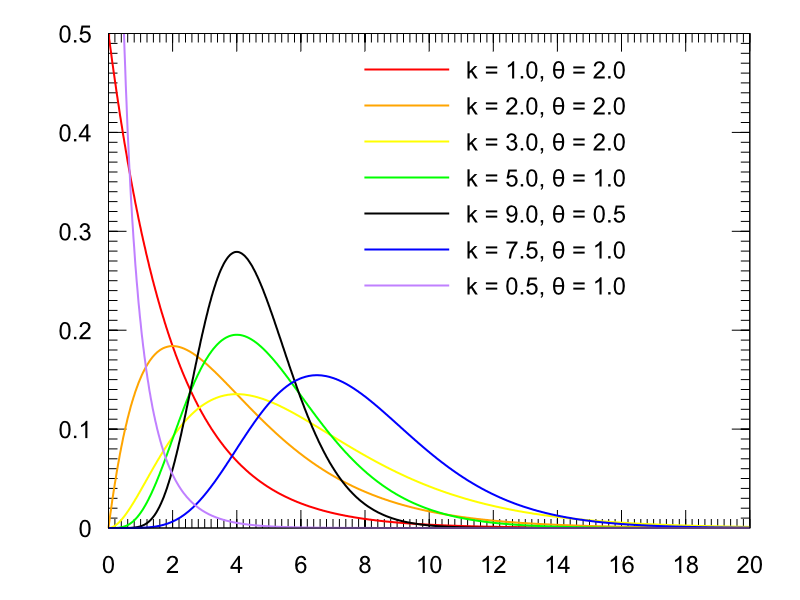
\includegraphics[width=0.5\linewidth]{Gamma_distribution.png} \end{center}

\begin{definition}[Gamma Distribution]\index{Gamma Distribution}
    A \term{gamma distribution} with \bred{shape parameter} $\alpha > 0$ and \bred{scale parameter} $\beta > 0$ for a continuous random variable $X$ has probability density function $$f(x) = \begin{cases} \frac{1}{\Gamma(\alpha)\beta^\alpha} x^{\alpha-1} e^{-\frac{x}{\beta}} & x > 0 \\ 0 & \text{otherwise} \end{cases}$$

    $X$ has mean and variance $$E(X) = \alpha\beta \qquad \qquad V(X) = \alpha\beta^2$$
\end{definition}

\textbf{Note:}

\begin{enumerate}\index{Gamma Function}
    \item $\Gamma(\alpha)$ is the \term{gamma function} defined by $$\Gamma(\alpha) = \int_0^\infty x^{\alpha-1}e^{-x} \,dx$$
    \item For $\alpha > 1$, $\Gamma(\alpha) = (\alpha - 1) \cdot \Gamma(\alpha - 1)$
    \item For $\alpha \in \mathbb{Z}_+$, $\Gamma(\alpha) = (\alpha - 1)!$
    \item $\Gamma\bracket{\frac{1}{2}} = \sqrt{\pi}$
    \item When $\alpha = 1$, $Gamma(1, \beta) = Exp(\beta)$. That is,k the exponential distribution is a special case of the gamma distribution\footnote{$\beta$ is the scale parameter, not rate -- recall scale $\theta$ and rate $\lambda$ from exponential distribution}.
    \item The sum of $n$ \bred{independent} $Exp(\theta)$ random variables $T = X_1 + X_2 + \cdots + X_n$, where $X_i \sim Exp(\theta)$, results in a gamma random variable with $T \sim \Gamma(n, \theta)$.
    \item The CDF of $\Gamma(\alpha, \beta)$ has no closed form when $\alpha, \beta \notin \mathbb{Z}_+$, making it difficult to compute probabilities without R. 
\end{enumerate}

{~~~}

Let's derive the expected value of Gamma.

Let $X$ be a random variable, $X \sim \Gamma(\alpha, \beta)$. 

Then, $f(x) = \begin{cases} \frac{1}{\Gamma(\alpha) \beta^\alpha} x^{\alpha-1} e^{-x/\beta} & x > 0 \\ 0 & \text{otherwise} \end{cases}$

$\allowdisplaybreaks \begin{aligned}[t]
    E(X) & = \int_0^\infty x \cdot f(x) \,dx                                                              \\
         & = \int_0^\infty \frac{1}{\Gamma(\alpha) \beta^\alpha} x^{\color{red} \alpha} e^{-x/\beta} \,dx \\
         & = \frac{1}{\Gamma(\alpha)\beta^\alpha} \int_0^\infty x^\alpha e^{-x/\beta} \,dx
         & \text{Let $u = \frac{x}{\beta}$, $dx = \beta \,du$}                                            \\
         & = \frac{1}{\Gamma(\alpha)\beta^\alpha} \int_0^\infty (u\beta)^\alpha e^{-u} \beta \,du         \\
         & = \frac{1}{\Gamma(\alpha)\beta^\alpha} \int_0^\infty \beta^{\alpha+1} u^\alpha e^{-u} \,du     \\
         & = \frac{\beta}{\Gamma(\alpha)} \int_0^\infty u^\alpha e^{-u} \,du
\end{aligned}$

\textbf{R Code Computation -- Gamma} 

Since the CDF of a gamma random variable has no closed form solution, we can use R statistical software to compute probabilities when $\alpha, \beta \notin \mathbb{Z}$. 

Given $X \sim \Gamma(\alpha, \beta) \dots$

\begin{itemize}
    \item $P (X \le k)$ is computed with \texttt{pgamma(k,shape=$\alpha$, scale=$\beta$)}. You MUST indicate whether you are using scale or rate parameters when using R since it allows for either: $\Gamma(shape, scale)$ or $\Gamma(shape, rate = \frac{1}{scale} = \frac{1}{\beta})$
    \item To simulate $n$ data values from $X$, we use \texttt{rgamma(n,shape=$\alpha$,scale=$\beta$)}
\end{itemize}

\begin{example}
    The number of service requests fulfilled by a technician at a support centre is Poisson distributed with an average of $10$ per workday (8 hours). How would you model the random time it takes to complete two unrelated and independent service requests by this technician? Find the probability that two service requests takes more than $3$ hours to fulfill.

    Let $R$ be the number of service requests per workday (8 hours). 

    $R \sim Pois(\lambda = 10)$. 

    Let $T_i$ be the time in hours to fulfill the $i$\textsuperscript{th} service request. 

    $T_i \sim Exp\bracket{\theta = \frac{8}{10}}$. 

    Want to model $Y = T_1 + T_2 \sim \Gamma(\alpha = 2, \beta = 0.8)$. 

    $f(y) = \begin{cases} \frac{1}{\Gamma(2) 0.8^2} y^{2-1} e^{-y/0.8} & y > 0 \\ 0 & \text{otherwise} \end{cases} = \begin{cases} \frac{1}{0.64} y e^{-y/0.8} & y > 0 \\ 0 & \text{otherwise} \end{cases}$

    $\begin{aligned}[t]
        P(Y > 3) & = \int_3^\infty \frac{1}{0.64} y e^{-y/0.8} \,dy                                          \\
                 & = \frac{1}{0.64} \int_3^\infty y e^{-y/0.8} \,dy                                          \\
                 & = \frac{1}{0.64} \left[ -0.8y e^{-y/0.8} - 0.64 e^{-y/0.8} \right] \bigg|_3^\infty        \\
                 & = \frac{1}{0.64} \left[ 0 - 0 + 0.8y e^{-3/0.8} + 0.64 e^{-3/0.8} \right] \bigg|_3^\infty \\
                 & \approx 11.17\%
    \end{aligned}$

    $\therefore$ There is $11.17\%$ chance that 2 service requests take more than 3 hours. 

    {~~~}

    Using R to compute $P(T > 3) = 1 - P(T \le 3)$, we use \texttt{1-pgamma(3,shape=2,scale=0.8)}. 
\end{example}

% TODO: Exact vs Chebyshev's Inequality (Week 9 pp.15-16)

\section{Percentile}

\begin{definition}[Percentile]\index{Percentile}
    The $k$\textsuperscript{th} percentile is the value of a random variable for which $k\%$ of values are less than or equal to it. For a random variable $X$ with PDF $f(x)$, the $k$\textsuperscript{th} percentile $x_{k/100}$ is the value of $X$ at which $k\%$ of outcomes lie below it. That is, $$P(X \le x_{k/100}) = \frac{k}{100} \qquad OR \qquad x_{k/100} = F^{-1} \left( \frac{k}{100} \right)$$
\end{definition}

\textbf{Special Percentiles}

\begin{itemize}
    \item The \term{median} is also called the $50$\textsuperscript{th} percentile
    \item The \term{first quartile} and \term{third quartile} are the $25$\textsuperscript{th} and $75$\textsuperscript{th} percentiles, respectively. 
    \item Measure of spread called \textrm{Inter Quartile Range} (IQR) $ = Q_3 - Q_1$. 
\end{itemize}

\begin{example}
    Find the median of a random variable $M$ with PDF $f(m) = 3m^2$, $0 \le m < 1$. 

    Let $m_{0.5}$ be the median. 

    $\begin{aligned}[t]
        \int_{0}^{m_{0.5}} 3m^2 \,dm & = 0.5           \\
        m^3 \bigg|_{0}^{m_{0.5}}     & = 0.5           \\
        {m_{0.5}}^3                  & = 0.5           \\
        m_{0.5}                      & = \sqrt[3]{0.5} \\
                                     & \approx 0.7937
    \end{aligned}$

    Thus, $50\%$ of the time, $M$ will take on a value larger than $0.7937$.
\end{example}

